% -*- coding: UTF-8 -*-
% lich_checklist_2017Q4.tex

\documentclass[UTF8,oneside]{ctexbook}

% \usepackage{xeCJK}
\usepackage[utf8]{inputenc}

% load paralist before enumitem
\usepackage{paralist}

\usepackage{hyperref}
\hypersetup{pdftex,colorlinks=true,allcolors=blue}
\usepackage{hypcap}

\usepackage{color}
\usepackage[usenames, dvipsnames, svgnames, table]{xcolor}
% \pagecolor{gray}

\usepackage{makeidx}
\makeindex

\usepackage{amsmath}
\usepackage{mathtools}

\usepackage{listings}
\usepackage{multicol}
\usepackage{fancybox}
\usepackage{tcolorbox}
\usepackage{enumitem}
\usepackage{multirow}
\usepackage{longtable}

\usepackage{indentfirst}

\lstset{%
    %alsolanguage=Java,
    %language={[ISO]C++}, %language为,还有{[Visual]C++}
    %alsolanguage=[ANSI]C, %可以添加很多个alsolanguage,如alsolanguage=matlab,alsolanguage=VHDL等
    %alsolanguage=tcl,
    %alsolanguage=XML,
    %alsolanguage=bash,
    tabsize=4, %
    frame=shadowbox, %把代码用带有阴影的框圈起来
    commentstyle=\color{red!50!green!50!blue!50},%浅灰色的注释
    rulesepcolor=\color{red!20!green!20!blue!20},%代码块边框为淡青色
    keywordstyle=\color{blue!90}\bfseries, %代码关键字的颜色为蓝色,粗体
    showstringspaces=false,%不显示代码字符串中间的空格标记
    stringstyle=\ttfamily, % 代码字符串的特殊格式
    keepspaces=true, %
    breakindent=22pt, %
    numbers=left,%左侧显示行号 往左靠,还可以为right,或none,即不加行号
    stepnumber=1,%若设置为2,则显示行号为1,3,5,即stepnumber为公差,默认stepnumber=1
    %numberstyle=\tiny, %行号字体用小号
    numberstyle={\color[RGB]{0,192,192}\tiny} ,%设置行号的大小,大小有tiny,scriptsize,footnotesize,small,normalsize,large等
    numbersep=8pt, %设置行号与代码的距离,默认是5pt
    basicstyle=\footnotesize, % 这句设置代码的大小
    showspaces=false, %
    flexiblecolumns=true, %
    breaklines=true, %对过长的代码自动换行
    breakautoindent=true,%
    breakindent=4em, %
    escapebegin=\begin{CJK*}{GBK}{hei},escapeend=\end{CJK*},
    aboveskip=1em, %代码块边框
    tabsize=2,
    showstringspaces=false, %不显示字符串中的空格
    backgroundcolor=\color[RGB]{245,245,244}, %代码背景色
    %backgroundcolor=\color[rgb]{0.91,0.91,0.91} %添加背景色
    escapeinside=``, %在``里显示中文
    %% added by http://bbs.ctex.org/viewthread.php?tid=53451
    fontadjust,
    captionpos=t,
    framextopmargin=2pt,framexbottommargin=2pt,abovecaptionskip=-3pt,belowcaptionskip=3pt,
    xleftmargin=4em,xrightmargin=4em, % 设定listing左右的空白
    texcl=true,
    % 设定中文冲突,断行,列模式,数学环境输入,listing数字的样式
    extendedchars=false,columns=flexible,mathescape=false
    % numbersep=-1em
}

\newenvironment{enumbox}[0]{
    \begin{tcolorbox}
    \begin{compactenum}
} {
    \end{compactenum}
    \end{tcolorbox}
}

\newenvironment{itembox}[0]{
    \begin{tcolorbox}
    \begin{compactitem}
} {
    \end{compactitem}
    \end{tcolorbox}
}

% table
\setlength{\arrayrulewidth}{1pt}
\setlength{\tabcolsep}{16pt}
%\renewcommand{\arraystretch}{1.5}
\newcolumntype{s}{>{\columncolor[HTML]{AAACED}} p{3cm}}

\arrayrulecolor[HTML]{DB5800}

\usepackage{tikz,mathpazo}
\usetikzlibrary{positioning, fit, matrix, shapes, arrows, chains, trees, arrows.meta}

% \bibliographystyle{plain}
% \bibliography{math}

\tikzset{%
  >={Latex[width=2mm,length=2mm]},
  % Specifications for style of nodes:
            base/.style = {rectangle, rounded corners, draw=black,
                           minimum width=4cm, minimum height=1cm,
                           text centered, font=\sffamily},
  activityStarts/.style = {base, fill=blue!30},
       startstop/.style = {base, fill=red!30},
    activityRuns/.style = {base, fill=green!30},
         process/.style = {base, minimum width=2.5cm, fill=orange!15,
                           font=\ttfamily},
}

% 摘录
\usepackage{verbatim}
\usepackage{libertine}
\usepackage{graphicx}
\usepackage{framed}

\newcommand*\openquote{\makebox(25,-22){\scalebox{5}{``}}}
\newcommand*\closequote{\makebox(25,-22){\scalebox{5}{''}}}
\colorlet{shadecolor}{Azure}

\makeatletter
\newif\if@right
\def\shadequote{\@righttrue\shadequote@i}
\def\shadequote@i{\begin{snugshade}\begin{quote}\openquote}
\def\endshadequote{%
\if@right\hfill\fi\closequote\end{quote}\end{snugshade}}
\@namedef{shadequote*}{\@rightfalse\shadequote@i}
\@namedef{endshadequote*}{\endshadequote}
\makeatother

\usepackage[normalem]{ulem}

\newcommand{\hl}{\bgroup\markoverwith
  {\textcolor{yellow}{\rule[-.5ex]{2pt}{2.5ex}}}\ULon}

%\usepackage{soul}

%\newcommand{\hlc}[2][yellow]{{%
%    \colorlet{foo}{#1}%
%    \sethlcolor{foo}\hl{#2}}%
%}

% todonode
\usepackage{lipsum}                     % Dummytext
\usepackage{xargs}                      % Use more than one optional parameter in a new commands
% 
\usepackage[colorinlistoftodos,prependcaption,textsize=tiny]{todonotes}
\newcommandx{\unsure}[2][1=]{\todo[linecolor=red,backgroundcolor=red!25,bordercolor=red,#1]{#2}}
\newcommandx{\change}[2][1=]{\todo[linecolor=blue,backgroundcolor=blue!25,bordercolor=blue,#1]{#2}}
\newcommandx{\info}[2][1=]{\todo[linecolor=OliveGreen,backgroundcolor=OliveGreen!25,bordercolor=OliveGreen,#1]{#2}}
\newcommandx{\improvement}[2][1=]{\todo[linecolor=Plum,backgroundcolor=Plum!25,bordercolor=Plum,#1]{#2}}
\newcommandx{\thiswillnotshow}[2][1=]{\todo[disable,#1]{#2}}
%

\usepackage[simplified]{pgf-umlcd}


\title{LICH技术指南}
\author{董冠军}
\date{\today}

\begin{document}

\maketitle
\tableofcontents

\chapter{导言}

\section{导言}

研判形势,淬炼心法,有所为,有所不为,乃至无为而无不为。

修道而保法,故能为胜败之政。

\begin{shadequote}

    道生一,一生二,二生三,三生万物。\\
    道生之,德蓄之,物形之,势成之。
\end{shadequote}

精一之学,体用兼备。
\begin{shadequote}

    天地之道,可一言而尽也:其为物不二,则其生物不测。\\
    天下之动,贞夫一者也。\\
    圣人抱一以为天下式。\\
    恒以一德。
\end{shadequote}

太极哲学,双线法则,圆点哲学,一分为三,提供了诸多值得反复体味的命题。

一,切己言之,就是事业,须更上一层楼。一是整体,是根据地,是不间断,也是突破点。

博厚,高明,悠久。

空灵之境,有无相生,有生于无。空非空寂,众缘所起,云行雨施,品物流行。

太极本无极。

上溯,万法归一,一归空。

五轮书,地水火风空。

建立自我,追求无我,是逆向工程。下学而上达。

\section{战略,或道}

\section{方法谈}

爱因斯坦说过这句话:我们不能用制造问题时同一水平的思维来解决问题。也许他意味着我们需要摆脱与我们对一个问题有关的消极的看法。如果我们对问题本身太投入,那么我们永远无法越过这个局面。

在一本叫“治愈与复原”中,David R. Hawkins详细阐述了这一点。他说,“问题最好不要在他们发生的同一水平上解决,而是在他们的上一个阶级上解决...通过超越他们,从更高的角度看待问题,问题很容易迎刃而解。
较高层次上,由于这种观点的转变,问题会自动解决,否则人们可能会看不到任何的问题。”

很多时候,我们面对一个问题时,总会把精力集中在问题上,一直问怎么“解决”呢?我们可能最终会走入死角,沮丧。
因为我们似乎找不到很好的解决办法。无论如何,不要把精力集中在问题本身上。花几分钟时间,花费你的时间和精力来正面地解析。
我们无法控制经常会有事情出现的,不要浪费时间担心这些事情;只花时间在你可以改变或控制的事情上。

\subsection{中庸}

\subsection{圆点哲学}
\subsection{双线法则}
\subsection{黄金分割率}
\subsection{80/20规则}
\subsection{黄金圈法则}

\subsection{达里奥的原则}

欲达到我们的目标,必须实事求是,客观公正地面对现实,正视自身的缺点和不足,而有以克服之。

这是真的吗?求真是第一位的,吾爱吾师,吾更爱真理。对道听途说的观念,我们固然要保持警觉和必要的批判精神。
对自我意识,也要慎思明辨。保持开放之心和专注之念,对自己的观念做压力测试,力求准确更准确。
而不能陷入先入之见,或自欺欺人,没有荣辱,只有是非。不当的虚荣心和自尊心会妨碍通向真正的目标。

对我们不知之物,保持谦卑,保持饥饿,保持愚蠢。

选择至关重要,我们必须承担选择的后果,为选择负起责任。
弱点,由弱点导致错误,皆在所难免。
但由此错误,吃一堑长一智,如果能通过反思而增强了自己,就是有益的。
从错误中学习,进步,进化,是通向成功的捷径。

任一选择,都带来其效应和影响。一阶效应也许不错,但二三阶效应可能已变形,
祸福相依,需要更多的洞见。关键的选择,决定了我们人生的质量。

成长,或曰进化,是唯一的目的。财富,名利皆是果,而不是因。
当我们围绕成长,而动心忍性,增益其所不能的时候,就是走在自我进化的路上。

自我进化,有一五步法可资遵循:
\begin{enumbox}
\item 设定清晰的目标
\item 觉知问题
\item 诊断问题
\item 设计方案
\item 执行方案
\end{enumbox}

五步法是迭代过程。每一步都需要投入必要的资源,做选择,做策划。

对比目标和输出的不同,找到不足,做出适当的调整,类似于PDCD。不妨想象,有台巨大的机器,作为输入输出的中介。
我们的核心任务,就是维持机器的良好运行和高效产出。

资源调度,采取开放的视角,并非一定需要我们亲力亲为。
我,即是设计者,也是执行者,主要作为设计者而存在。
任何人都非全知全能,而是有长有短,管理者的职责,在于知人善任。

不必为自己的弱点而沮丧,君子性非异也,善假于物。

唯一的目的,就是自我进化。唯一的事,就是打造机器。
机器是我们拥有的容器,即是心法,也是产品。我们是机器的架构师。

单纯观念,不足以动人。做出作品,持续产出,才能实现自我价值,立于不败之地。

实有诸己之谓德。默默地完成进化,是最明智的选择。围绕选定的一,厚积薄发,静水深流。

道生一,一即是战略,也是方法。

原则,架构起了价值和行动的桥梁。让我们有所遵循,持续积累,而不是茫然无措,本末倒置。

佛陀的教导

以戒为师。戒可释为原则,或良好习惯。

大乘起信论的一心二门的义理架构,予人深刻启示。

达里奥与王阳明

良知是比原则更基础的范畴,良知是一种元认知能力。
致吾心良知于事事物物,则事事物物皆得其理。

达里奥求真的意志和可操作性,较阳明为突出。
资本主义的熏陶,更适应于现实人生。

毛主席在其著作中,深入分析了认识的各种问题,如主观主义,教条主义,经验主义,
统称为主观主义,即主客观的分裂和不一致。以此指导行动,则误导行动。

马利克的管理学,采用系统论,控制论和仿生学等知识,以应对现实世界的复杂性。



RAS

多快好省

\part{硬件抽象层}
\chapter{硬件抽象层}

4+1


\part{存储引擎层}
\chapter{架构}

\section{RAID分析}

RAID分析作为架构驱动力

假设和信念
\begin{enumbox}
\item 云是新常态
\item 数据资产是战略资源
\item 全闪是大势所趋
\end{enumbox}

新设计解决了什么老问题?
\begin{enumbox}
\item 单卷的水平扩展问题
\item IO path上的数据转发问题
\item allocate性能低,影响精简配置和COW性能
\item 每个节点导出core、disk等资源,进行全局调度(均衡)
\item 灵活的MM
\item thread local影响CPU利用率
\item ***
\item 重新调整数据布局
\item 单卷大小的限制(支持大卷)
\item chkinfo是动态大小的,副本数、EC配置
\item 底层chunk对象依然不是跨卷的
\item ***
\item COW: volume和snapshot共享对象
\item ***
\item table1/table2实现过于复杂的问题
\item disk md and slots
\item coroutine难于调试
\item ***
\item 多网络
\item MULTIPATH
\item IPv6
\end{enumbox}

\section{模块}

分布式系统架构通常包括几个部分:client、mds、cds。分别对应什么?
\begin{center}
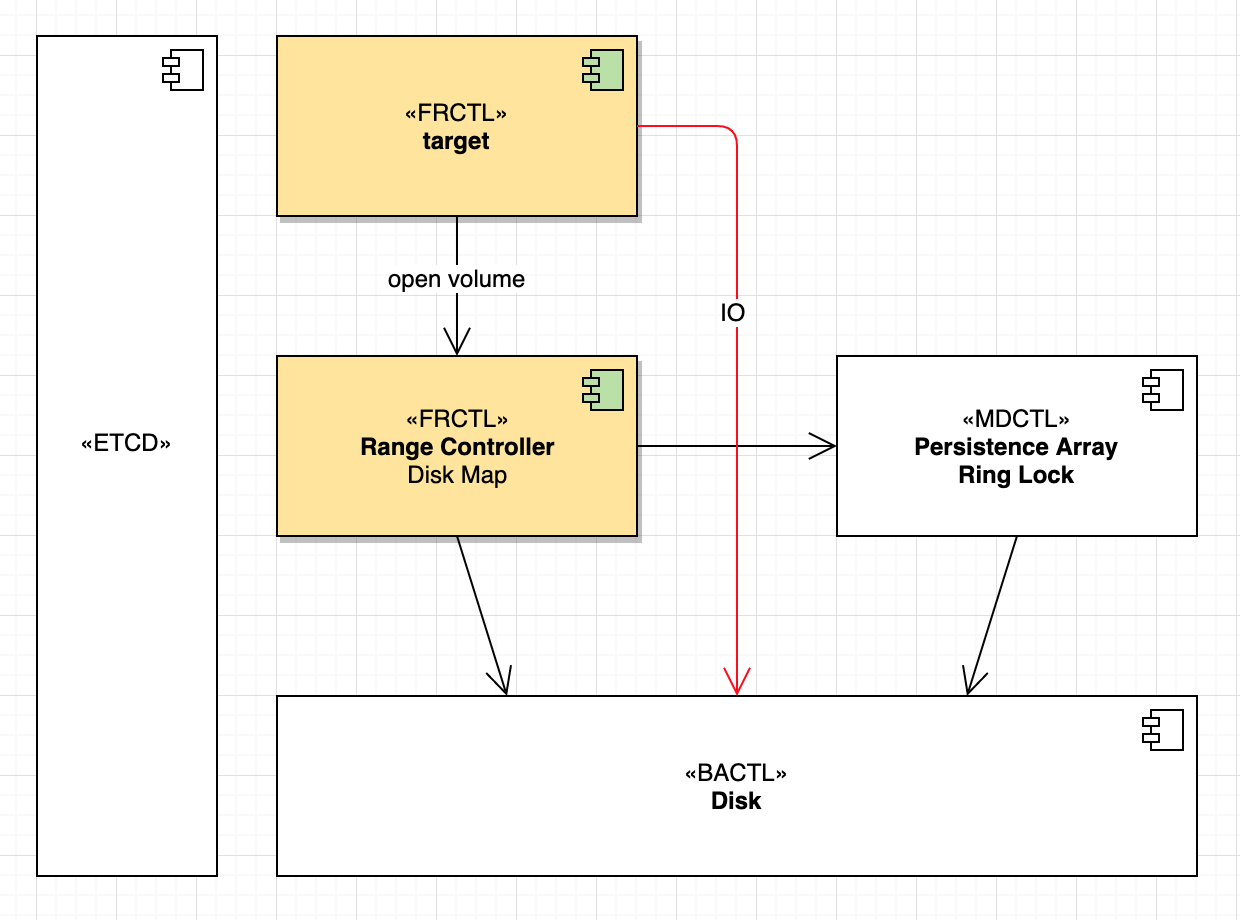
\includegraphics[width=11cm]{../imgs/modules.png}
\end{center}

target到bactl,有两条路径,视是否通过range ctl而定。如果不通过range ctl(rangectl bypass),数据流可直达后端存储,
实现控制流和数据流分流的目的。同时降低了转发成本。

问题集:
\begin{enumbox}
\item 为什么range ctl和mds是分离的进程?
\item vss是否必要?
\item ***
\item io路径是什么?
\item 副本一致性是如何实现的?
\item IO和Recovery之间如何同步?
\end{enumbox}

\subsection{FRCTL}

target如何与分布式卷相连?

vss包括4个range,range包括4个pa,pa包括固定数目的chunk。pa和chunk都是4M大小。
\todo{vss是否必要}vss是否必要,还是增加了设计复杂度?

token是向range ctl获取的,粒度为chunk。range ctl上每个chunk维护有token计数器。

token里包含了每个副本的位置信息,这是向mds请求得到的。

client并不与mds直接通信。分离fr和mds为两个进程,一是可以指定不同的core;二,便于debug。

\begin{center}
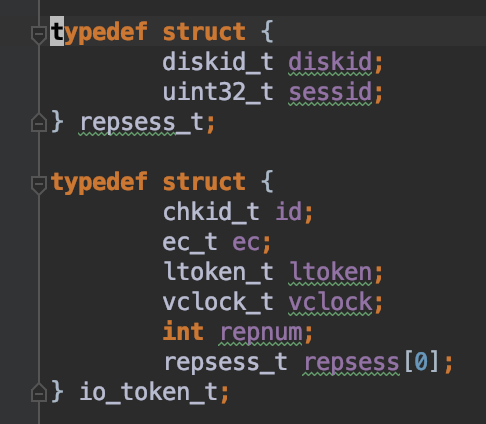
\includegraphics{../imgs/token.png}
\end{center}

range ctl和mds都在hash ring上。都采用了hash机制来定位目标节点。
所以\hl{有两个hash ring:range ctl和mds}。两个ring都通过mds master来维护。
ring的节点结构是什么?node and core?
\begin{center}
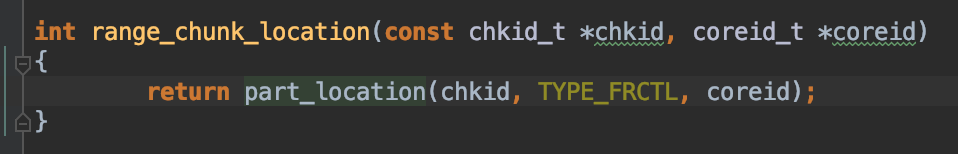
\includegraphics[width=11cm]{../imgs/chunk-location.png}
\end{center}

partition是range ctl和mdctl共用模块。range ctl目前归属frctl。

lease机制目前没用,如果需要把range ctl放置到session所在的位置(一个volume的所有range都在一个节点上?),
可以选用lease机制,而不用dht机制。怎么理解session?

一旦ring结构发生变化,会有什么影响?SSAN通过epoch来管理ring结构的变化。

ring上节点负载均匀性如何?

ring lock有什么用?在mds master上维护状态,处理ring发生变更的情况。
是否可通过引入epoch实现同样的功能?

GFM?解决全局同一视图的问题。

如何识别和处理stale消息?

\subsection{MDCTL}

hash ring上有一个节点充当master角色。如何选主,如何保持其唯一性?
通过etcd lock实现。

\subsection{BACTL}

diskid是全局的,在etcd上有目录。

\subsection{Driver}

diskmd磁盘访问接口,支持libnvme驱动。

需要管理物理内存,如hugepage和memory pool。

NVMe/RDMA需要访问物理内存。

\section{资源}

从\hl{资源的生命周期模型}开始思考。资源包括:\hl{集群、节点、core、磁盘、pool、volume、snapshot}等,以及内部资源。

ERD

\subsection{Cluster}

\subsection{Node}

Node是Process、Core、Disk等资源的合集。利用Core的方式是个亮点。

增删节点是重大事件

\subsection{Disk}

Disk导出,分配过程可以进行全局调度。

调度器位于md ctl。md ctl负责管理chkid到disk id的映射关系。
\todo{diskid类型}diskid采用16bit整数是否太小?

diskmap.c,不宜放入bactl。bactl所有API都带diskid,针对单盘进行。

怎么做到每个副本属于不同的节点的呢?

如何管理diskmap的版本呢?

\hl{数据分布的均匀性}: 节点和磁盘两种粒度

tier and cache?

负载均衡

\subsection{Pool}

\subsection{Volume}

\begin{enumbox}
\item TP
\item Recovery
\item Balance
\item QoS
\item ***
\item EC
\item Dedup
\item Compress
\item ***
\item RC
\end{enumbox}

\subsection{Snapshot}

如何共享底层对象?

consistency group

分析各种操作的复杂度,包括空间和时间。

\hrulefill

平安科技:可写快照

与COW平列实现ROW?

快照占据底层volume空间共享?

COW的问题
\begin{enumbox}
\item 影响写性能
\item Rollback慢
\item clone卷慢,scan snap tree。snapshot也可执行flatten
\end{enumbox}

snap头包含什么指针?

快照卷与物理卷什么对应关系,

映射表的管理粒度,是chunk还是page?范围,是全局还是私有?

COW一次读,两次写

ROW一次读,一次写

\hrulefill

SSAN的snapshot实现。

ROW,两层元数据?

vol id发生变化,凡是依赖于vol id的都需要进行适配。

\section{数据}

\subsection{ETCD}

\subsection{卷的元数据}

两层元数据,etcd指向顶层对象。每个对象属于一个卷,
因为不是一般的对象系统,\hl{在快照的情况下,无法直接共享}。

\chapter{模型}

\begin{tikzpicture}[show background grid]
    \begin{class}{Disk}{6, 0}
    \end{class}
    \begin{class}{Pool}{6, 2}
    \end{class}
    \begin{class}{Volume}{6, 4}
    \end{class}
    \begin{class}{Host}{6, 6}
    \end{class}
    \begin{class}{Cluster}{0, 2}
    \end{class}
    \begin{class}{Snapshot}{0, 4}
    \end{class}

    \composition{Cluster}{pools}{1..*}{Pool}
    \composition{Pool}{disks}{1..*}{Disk}
    \composition{Pool}{volumes}{1..*}{Volume}
    \composition{Volume}{mapping}{*..*}{Host}
    \composition{Volume}{snapshots}{1..*}{Snapshot}
\end{tikzpicture}

\section{Cluster}

整体

\section{Pool}

把物理节点划分为不同的保护域,一个卷的所有数据只出现在一个保护域内。卷可以跨保护域进行复制和迁移。

默认一个,包括所有节点。

% 保护域是物理节点的划分,存储池是存储介质的划分。每块盘只能出现在一个存储池里。

Pool: 逻辑容器

故障域有粒度之分,如磁盘,节点,机架,机柜,数据中心。

存储池内,要满足故障域规则:一个chunk的不同副本,分布在不同的故障域内。\label{rule:faultset}

在初次分配,再平衡和恢复等过程中,都需遵循这些规则。

\begin{tcolorbox}

可以参考ceph的CRUSH实现。bucket和device定义了集群的物理拓扑结构,rule定义了数据存取规则,
pool上关联rule,从而定义了pool中卷数据的放置规则。设备即OSD,对应一个物理磁盘。

***

存储池可以取代保护域,定义所有对象的存放位置是一个节点集。

***

存储池可以用来实现tier cache。重定向IO到cache pool。

***

统一概念:保护域,故障域,存储池,pool。Consistency Group不同于pool,与物理存取无关,
而是卷的逻辑集合,卷可以来自不同的pool。

\end{tcolorbox}

与存储池有什么同和异?存储池可以看做关联了磁盘的pool,可以看做pool的子类。

属性:
\begin{enumbox}
\item 配额
\item 复制类型:副本 OR EC
\item 磁盘列表
\item 定义精简池
\item 存储池上可以指定卷的副本数
\item \hl{有足够的故障域,且不同故障域配置一致的资源量}
\end{enumbox}

操作:
\begin{enumbox}
\item 创建
\item 删除
\item 扩展(添加磁盘到\hl{已存在的存储池},该映射关系持久化到本地,同步到admin节点)
\item 缩容(从存储池中移除磁盘,引发数据重建过程)
\item \hl{自动或手动按磁盘速率进行存储池分级划分}
\item 不同存储池之间,卷的复制
\item 不同存储池之间,卷的迁移,可在线或离线
\item 存储池级别的统计信息
\end{enumbox}

% 存储池是disk的集合,与节点无关。但disk所在的节点构成存储池的节点列表,不同存储池的节点可能覆盖。

存储池下,可以创建volume。没有关联磁盘的存储池,不能创建卷。

\hl{chunkid到磁盘物理位置有两级映射:chunk的副本节点列表,节点内chunkid到物理地址的映射}。

在为卷分配chunk的时候,需要确定各个副本的物理存储位置。当前实现是返回不同副本的节点列表。
如果指定了存储池,就需要在存储池所在的节点范围内进行分配。同时要满足故障域和数据均衡规则。

\begin{tcolorbox}
移动采集中存储池要求,相比于目前的逻辑pool,更多是一种设计上的退步。
存储虚拟化的目标,是物理位置无关。我们可以基于逻辑容器,实现基于策略的管理。
所以,\hl{从实现层面,要保留当前pool的功能,按照系统配置确定pool的类型}。
\end{tcolorbox}

% 存储池内,要满足故障域规则(\ref{rule:faultset})

步骤:
\begin{enumbox}
\item 创建pool,但此时不能创建pool的元数据chunk,因为还没有绑定磁盘(需要一全局的地方,存储pool名字)
\item 添加磁盘到pool,通知admin节点
\item 当在pool下面创建卷的时候,前提条件是已准备好磁盘,生成pool元数据chunk(位于同一pool里)。
\end{enumbox}

pool元数据chunk必须位于自己的存储池内,如果分布在不同的存储池,不满足故障域条件。

pool引导信息可以存在rootable里。

\section{Volume}

属性:

操作:
\begin{compactenum}
    \item rename
    \item resize \info{在线扩容}
    \item mv
    \item copy \change{全量拷贝/增量拷贝} \change{跨存储池拷贝} % change不能出现在box里
\end{compactenum}

\section{Snapshot}

snapshot隶属于卷,无卷则无快照,快照组织成快照树,其中有且只有一个快照是可写快照,即卷的写入点。

\section{Mapping}

数据隔离/ACL,数据保护

卷对主机的可见性。一个卷只有映射给了某主机,才可以被该主机访问。


\section{Consistency Group}

一致性卷组

\begin{shadequote}
Consistency Groups could be useful for Data Protection (snapshots, backups) and
Remote Replication (Mirroring).

The Mirroring support will allow to setup mirroring of multiple volumes in the
same consistency group (i.e. attaching multiple RBD images to the same journal
to ensure consistent replay).

There is already an interest to implement this functionality as a part Mirroring feature:
http://tracker.ceph.com/issues/13295

The snapshot support will allow snapshots of multiple volumes in the same
consistency group to be taken at the same point-in-time to ensure data
consistency.
\end{shadequote}

\chapter{元数据管理}

etcd,存储池,目录,卷,快照,映射

结合lsv,row snapshot考虑当前的元数据管理,看看会有哪些瓶颈?

\section{元数据}

最重要是chkinfo结构体,表示一个chunk的若干属性,包括副本位置信息。

区分磁盘结构和内存结构。

三级元数据。是一颗大树。集群/存储池/目录/卷/chunk/replica。

\section{一致性协议}

元数据和数据的更新方式为何不同?

块存储的顺序一致性要求。成功返回的各副本强一致性,
不成功返回的,各副本可能处在不一致的状态,且无需修复。

元数据是否会进入某种不一致的状态?在整体掉电的情况下。

sqlite错误记录,指向无效的chunk?

元数据写入是sync的

事务操作,简单模型和组合模型。

\subsection{clock的作用}

分析三部曲:先分析正常情况,后分析并发场景,然后分析异常情况,
有各种各样的故障,逐一加以说明。

正常情况下,用clock维护一个chunk各副本的一致性。

每次io,携带有clock,即是chkstat.chkstat\_clock。在副本级,维护有chkid到<clock,dirty>的映射关系。
每个副本按clock递增(+1)的顺序写入。

重新载入卷,chkstat.chk\_clock设为0。

恢复一个卷的顺序,影响到并发度。

chkstat.chkstat\_clock与replica.clock相等时,说明本次IO写入完成。

写入过程,副本上的io更新序,wlist。

chunk.clock与replica.clock有双向同步的关系。一开始,chunk.clock=0,随着io.clock传播到各副本。
各副本按io.clock的递增顺序,依次完成每个io。重新加载时,通过fully过程,选择一clean副本,
并令chunk.clock=replica.clock,并以该副本为基准,对比修复余下的副本。在写入都正常完成的情况下,
chunk.clock恒等于各副本clock。

各副本写入前,let dirty=1;写入完成后,let dirty=0。通过此标记位来跟踪clock状态。

RM就地编辑,没有记录日志,所以无法应用REDO/UNDO恢复策略。
对已应答的记录,执行REDO策略;对未应答的记录,执行UNDO策略。

更新chunk.clock后,如果没有成功地传播到副本上,则该chunk上的写不可继续。

\hl{元数据采用与raw一样的一致性等级,是否合理}? 写meta和raw不同,与此有关?

\subsection{若干故障情况}

每个chunk的各副本,状态由几部分构成:卷控制器上的chkinfo和chkstat,
replica级别的clock信息,网络ltime。

分析每一个条件:
\begin{compactenum}
\item offline
\item reset (ltime是与nid的网络连接状态,异常时重置)
\item replica status
\item chkstat.chkstat\_clock (chunk级,io级,不需持久化,每次重启设为0)
\item clock and its dirty status
\end{compactenum}

一个节点clock丢失,所有写流程都会到达这个节点(拔盘的情况与此类似)

在chunk\_push前,会从replica上同步clockstat,然后对比。

一个副本clock丢失

所有clock丢失

重启整个系统,

\section{分配}

精简配置

\section{回收}

\section{加载}

\section{恢复}

\section{均衡}

\chapter{关键过程}

过程分析分两种:正常情况和异常情况。特别是故障情况下,过程之间存在广泛的交互作用,变得更为复杂。

过程需要具备一些重要属性,如事务ACID,safety和liveness等,要具体情况具体分析。
值得注意的是,若干过程需要实现为可重入的。

其它注意事项:
\begin{compactenum}
\item 必须正确处理过程的返回值。
\item 一定要检查加锁的返回值,返回值失败,不能unlock,从而保证加锁解锁的对称性
\item 资源的分配和释放,使用goto方法,用stack方式管理
\item 过程运行在协程内,还是协程外?
\item 变量作用域,在作用域以外访问变量
\item 过程是否并发安全?
\item 过程执行时间是否过长,且中间无中断?比如有大循环,有同步IO操作等
\end{compactenum}

实体有复合和简单之分。简单实体的基本操作包括增删改查,复合实体在此基础上多出了子节点的相关操作。

按一颗树来组织,简单实体是叶子节点,复合实体是中间节点或根节点。

if-then/what-if假设分析:
\begin{compactenum}
\item 资源管理的对称性(分配/释放, 资源包括fd,lock,malloc等)
\item 如果此处发生故障,会如何?容错
\item 如果有多个task进入,会如何?并发
\item 会有什么不良影响吗?safety
\item 过程能完成吗?liveness
\end{compactenum}

事务分析:
\begin{compactenum}
\item 可串行化(两阶段锁,树协议)
\item 事务日志:持久化每一个操作,包括必须的上下文信息
\item 重启时,REDO/UNDO(原子性)
\item 为减少需要REDO的操作,记录检查点
\end{compactenum}

\section{集群}

\subsection{加入节点}

\subsection{删除节点}

\section{存储池}

\subsection{创建存储池}

\subsection{删除存储池}

\subsection{添加磁盘}

% \subsection{添加缓存盘}

\subsection{删除磁盘}

拔盘会产生一系列的影响,如IO抖动,控制器主副本丢失,存储池降级等。
与读写,控制器切换,QoS策略,恢复,平衡等过程都有密切关系。

\begin{compactenum}
\item 更高效的检测方法
\item 何时关闭fd,应避免fd重用造成的影响
\item 如何降低check过程对性能的干扰
\item lich health clean是否可以自动化
\item 盘会不会重新加入,从而造成副本数增多
\item RAID的影响,干扰别的盘,造成IO中断
\item rescan,不必等到下次恢复周期
\end{compactenum}

diskid字段上加索引

\subsection{空间分配}

admin维护着集群的拓扑结构。

故障域规则

分两层:副本的节点位置和副本的磁盘位置。

注意多个chunk的局部性对性能和恢复性能的影响。

\section{目录}

\section{卷}

卷属性:
\begin{lstlisting}
- 副本数
- 精简配置
- 当前链接
\end{lstlisting}

\subsection{创建卷}

\subsection{删除卷}

\subsection{加载卷}

\begin{compactenum}
\item 延迟加载table2
\item 预加载table2
\item 获取allocate属性的方式和性能
\end{compactenum}

\subsection{分配卷空间}

局部性

\subsection{unmap卷空间}

\subsection{查询卷属性}

\subsection{计算卷md5sum}

存在不能返回的情况

\subsection{resize}

扩容,不允许缩容

\subsection{rename}

前置条件:不能跨存储池

\subsection{拷贝}

两种实现方式:读写,基于快照

考虑在server端做!

可控的并发度

前置条件和后置条件

不变式

\subsection{迁移}

同池迁移,同rename

跨池迁移,前置条件

\subsection{切换卷控制器}

\begin{compactenum}
\item 源端volume\_proto是怎么回收的?
\item lease机制怎么影响本过程?
\end{compactenum}

\subsection{write}

\subsection{read}

\section{快照}

\subsection{创建快照}

\subsection{删除快照}

\subsection{回滚快照}

\subsection{克隆}

克隆卷后,需要保护其源快照。目前,克隆关系是单向的,克隆卷记录了其源快照信息,快照没有记录克隆卷的信息。

\subsection{FLATTEN}

\section{主机映射}

\section{后台任务}

\subsection{监控磁盘状态}

\subsection{恢复}

局部性

恢复性能与批量分配有关。如果连续的chunk,被分配到部分节点的部分盘上,就会影响到恢复性能。
恢复是按卷顺序扫描,调整该顺序,可以提高并行度。

删除卷

QoS,slow start

恢复要能有效处理多种故障情况,做到高效及时,QoS。

拔盘时,通过chunk\_check过程进行恢复。读发生在多个节点上,写发生在拔的盘所在节点(?)。
如果该节点盘较少,会影响到恢复性能。

\subsection{平衡}

平衡分控制器平衡和数据平衡。

卷在节点间和节点内的平衡,节点内core间平衡,可以引入一hash table来解决,
带来的问题是什么?可以容易地克服吗?

通过迁移控制器来实现卷在节点和corenet上的平衡。每个corenet指的是各个节点上具有相同core hash的core组成的网络。

平衡算法要保证输出的稳定性,分两阶段:定位和迁移。定位阶段确定所有卷控制器的位置,每个卷最多迁移一次。

\subsection{回收卷}

\subsection{回收快照}

\subsection{恢复快照}

\subsection{FLAT卷}

flat性能分析:读,分配,写多个阶段。能否批处理?并发度如何?

快照树

精简配置

删除卷

因为table2的写入特性,顺序处理各个chunk,并发度不高。

分布式并发?

属性依赖性:source < clone < flat。生成顺序是顺序的,flat完成后的重置顺序则是逆序的。
一般的事务过程,各阶段的顺序,也许按依赖性进行分析。无依赖的,理论上是可以并发的。
分布式系统的因果序,happen-before关系。

\subsection{存储池状态}

\begin{compactitem}
\item Available
\item Degraded
\item Readonly
\item Unavailable
\end{compactitem}

异步处理

cron后台执行一定的策略,如nagios等监控系统,处理结果放入/dev/shm

时间戳

pending状态

\chapter{核心数据结构}

\section{ETCD}

集群状态

\section{元数据管理}

对象标识和寻址机制

\section{SQLITE}

异步化

\section{DISK BITMAP}

空间分配器

\section{LEASE}

\section{CLOCK}

副本数据一致性

\section{MSGQUEUE}

离线消息处理

异步化,是否可提取出异步化框架?

\section{控制器缓存}

采用引用计数技术。

控制器切换和平衡

\section{副本缓存}

\section{扩展属性}

\section{快照}

\section{克隆卷}

\section{CORE AND Scheduler}

每个core有独立scheduler。为了与其它节点上的core进行通信,抽象出了corenet的概念。

实体标识和命名:hostname,nid,core hash,sockid。

RPC有发送端和接收端。

\chapter{运行时结构}

\section{CORE}

\subsection{\_\_core\_worker}

\section{磁盘管理}

\subsection{diskctl\_start}


% malloc/gc, recovery, balance

\part{存储特性层}
\chapter{精简配置}

\chapter{EC}

\chapter{缓存}

\section{Redis Cache}

卷控制器所在节点,IO入口处,分页。当切换卷控制器的时候,清空redis cache。

采用redis LRU或FRU算法。

\begin{compactitem}
    \item \verb|volume_proto_write|
    \item \verb|volume_proto_read|
\end{compactitem}

read过程,从io的两段向中间压缩,选取中间最大的加载区。

若发生volume controller切换,源端能否及时感知该事件,会有清理过程吗?怎么使源端的cache数据失效?
在cache里,有两级检查机制:卷和页。有总开关,分级,如果设定卷级状态失效,则全体页也是失效的。

为什么会发生volume controller切换?主动move,节点故障,iscsi session切换等。

切走,失效化,切回。如果在切回之前没有失效化,则有\hl{cache一致性问题}。

如何检测到该事件?

\begin{tcolorbox}
每发生一次切换,\verb|info_version|即+1,在redis key里加入该信息。
利用redis自身的置换机制,则切换不会造成cache一致性问题。
\end{tcolorbox}

\begin{compactenum}
\item config: \hl{功能开关}
\item 初始化
\item \verb|info_version|
\item 并发
\item 内存copy
\item batch update redis (mset and mget)
\item 存在,则不kset?
\item redis连接可以用unix domain,相比tcp方式提速1倍左右
\end{compactenum}

遗留问题:
\begin{enumbox}
\item 顺序读,分页后,性能下降
\item 随机读,破坏局部性
\item 内存cache?
\item 必须考虑基准性能,SSD read和redis read,IOPS哪个多?
\item \hl{快照回滚对cache的影响}
\end{enumbox}

即使是连接本地redis,tcp开销也是很大的,最多3w IOPS。如果缓存命中率低,或者分页引起的tcp开销,反而会导致读写性能下降。

实现cache有一些通用问题和瓶颈,可以提前指出。

\section{SSD Cache}

特性开关:xattr writeback

入口:\verb|writeback_commit|

节点级别,在添加磁盘时指定\hl{--cache}选项,即创建了SSD cache盘。

journalling? 优化随机IO。写入WAL即可返回。

所有非\verb|__FILE_ATTR_DIRECT__| IO,都流经SSD cache,由QoS机制控制流入流出的速率,达到流入流出的平衡。
同时,通过异步线程flush ssd cache的内容到目标位置。

与分层有什么不同:
\begin{compactitem}
\item IO路径(包括入口)
\item 目标位置
\item 容量
\end{compactitem}

tier考虑了热点数据,tier层容量计入总容量,cache层容量不计入总容量。

\subsection{BUG}

BUG: ssd cache假定io 512对齐。如果有非512对齐的IO,会产生core。

\chapter{Tier}

\chapter{QOS}

\section{概述}

学习的方法:
\begin{enumbox}
\item \hl{对标}:行业的标准做法是什么?
\item 如何才能更好地学习?
\item *
\item 先选出几篇经典论文,顺藤摸瓜,建立相关的知识体系。
\item 与专业人士交流,获取有价值的线索。
\item 还需要主动去悟,提问、消化、守破离,推陈出新
\end{enumbox}

参考网络QoS,存储QoS的核心算法与网络QoS相同。

集中式控制、分布式控制

排队论

态势感知?

在高IOPS的情况,QoS的开销过大,极大地拉低了性能,这是不可接受的。

每次请求都要获取一次时间,是不是必要的?

\subsection{参考}

\begin{enumbox}
\item OS中进程、线程调度算法
\item Disk IO调度算法
\item VM IO调度算法
\item Network QoS and Storage QoS
\item TCP/IP
\item iSCSI
\item SPDK QoS
\item Ceph dmClock
\item SolidFire QoS
\end{enumbox}

\section{算法}

采用了两种曲线

开放控制参数

比较指标:理论和实测值的距离,\hl{也可以考虑夹角的大小}。\change{距离函数}

底层采用token bucket,需要能容忍一定的jitter。

在调度器内加入QoS控制逻辑的设想: 每个core调度器对应一个或若干卷控制器。基于优先级队列,由core线程处理队列(scheduler队列?)。
每个卷控制器在对应的scheduler上注册自己的队列(IO任务、恢复任务)。 \hl{core上的每个卷,向scheduler注册自己,从而实现解耦}。
调度器不仅可以处理单个卷的QoS,也可以处理多个卷的QoS。

\hl{队列和线程}往往紧密结合为一体,参见SEDA、actor。

\hl{多mode调度器},根据实际负载条件动态地调整调度器策略。

何时从请求队列移入调度队列是QoS调度器的中心任务。

% \section{Quota}

\chapter{快照和克隆}

\chapter{灾备}

目前收集到的信息:

\begin{compactenum}
\item 方案1:forward 控制流和数据流,故障情况下异步传输
\item 方案2:基于libiscsi和iscsi协议(张胜玉提供,以前做过相关功能)
\item 方案3:老王提供的方案,先写入远程站点,故障情况下,从本地站点全量flush到远程站点
\end{compactenum}

中科院魏征当时实现了一部分,没有完成,类似方案1,考虑这部分代码是否可以复用。

主要的困难:
\begin{compactenum}
\item 选择网络拓扑,传输协议,复制策略
\item 控制流/数据流的保序
\item 故障处理
\item failover
\item 传输性能
\end{compactenum}

\begin{lstlisting}
我解释下iscsi的优势:
1. 我们系统本身就支持了iscsi server,因此无需再去实现一套server,实现一套server需要额外的代码,关键是对应的管理功能
2. 我们可以利用scsi协议预留给厂商的指令,封装一些控制指令(比如建立快照等)很好保证时序。
3. 有利于将来扩展,相比以上两点,这个重要性更高,因为我们的系统对外不管是iscsi,iser还是光纤,
最后里面都是要走scsi协议,一些scsi协议需要redirect到远端。如果不用这个方案,需要每个特殊命令单独实现一个同步指令。

控制流/数据流的保序,iscsi本身有时序处理
- 故障处理   - failover, 发生中断要进行本地记录增量日志,待恢复后将数据刷过去。
- 传输性能, iscsi协议本身无此瓶颈。
\end{lstlisting}

业务流量和复制流量隔离

多复制流量多通路


\part{存储协议层}
\chapter{iSCSI}

\section{IQN}

关于iqn的不变性,iqn是卷的公开标示,供上层应用引用该卷。改变iqn,需要通知依赖于iqn的应用,做出相应的改变。

回到lich的情况,iqn包含了路径部分:<pool\_name>.<image\_name>,跨存储池迁移,rename等操作会改变路径部分。

问题: 可否用卷的volid作为iqn的一部分,替代path,同时保证volid在各种操作下具有不变性?

ceph的做法:
\begin{compactenum}
\item rbd访问方式,用的是路径。
\item 通过tgt提供iscsi服务时,通过tgt配置项建立iqn到path的映射
\end{compactenum}

\begin{lstlisting}[frame=single]
<target iqn.2014-04.rbdstore.example.com:iscsi>
    driver iscsi
    bs-type rbd
    # Format is <iscsi-pool>/<iscsi-rbd-image>
    backing-store iscsi/iscsi-rbd  
    initiator-address <clients address allowed>
</target>
\end{lstlisting}

\section{CHAP}

In function \verb|ns_build_auth_chap|
\begin{compactitem}
\item \verb|lich_system_username|
\item \verb|lich_system_password|
\end{compactitem}

\section{白名单}

\begin{compactitem}
\item \verb|is_connect_allowed|
\end{compactitem}

没有设置ip或initiator,默认拥有全部权限,不符合白名单语义,最小权限原则。

xattr用于保持ip或initiator白名单,如果很长,则溢出。
需要找到更合适的存储方式。

\section{Initiator}

\begin{lstlisting}[language=bash,frame=single]
echo 2 > /sys/block/sdd/device/queue_depth
cat /etc/iscsi/initiatorname.iscsi
\end{lstlisting}

\chapter{NBD}


% RDMA, SPDK

\part{管理和应用}

\chapter{UMP}

\chapter{OpenStack}

\chapter{VMWare}


\part{公共构造块}
\chapter{标准库}

\section{CPU}

\subsection{pthread}
\subsection{coroutine}

\section{Memory}

\subsection{ymalloc}
\subsection{mem\_cache}
\subsection{mbuffer}

\section{Disk}

\subsection{Local File and Directory}
\subsection{AIO}

\section{Network}

\subsection{minirpc}
\subsection{rpc}
\subsection{corerpc}

\section{String}
\section{List}
\section{Hash}
\section{Skip List}
\section{Cache with ref}
\section{Date and Time}
\section{JSON}
\section{Lease}
\section{ETCD}


\part{工具和流程}
\chapter{LICH系统故障排查检查表}

\section{故障诊断}

故障诊断要结合集群和节点状态,core,日志,硬件,数据等因素。

\subsection{检查集群健康状态}

\begin{lstlisting}
# 节点列表,检查latency,uptime, nid等
lich list -v

# 节点,存储池和容量
lich stat

# 检查恢复状态
lich health
\end{lstlisting}

\subsection{检查ETCD}

\begin{lstlisting}
# etcd状态
etcdctl ls -r

# 版本
\end{lstlisting}

\subsection{检查系统时间}

\subsection{检查lichd版本}

\subsection{检查网络服务}

检查网络服务:ssh,ssh会影响到很多关键过程。
如果ssh连接过慢,引起超时异常。

\subsection{检查卷控制器的平衡性}

\begin{lstlisting}
# 节点间平衡
lich.balance --scan
lich.balance --balance

# 节点内core平衡
\end{lstlisting}

\subsection{查看CORE}

\begin{lstlisting}
./lscore.sh
\end{lstlisting}

\subsection{查看日志}

必要时,开启backtrace

必要时,开启DBUG日志等级

\subsection{检查硬件和操作系统状态}

CPU,内存,磁盘和网络

\subsubsection{磁盘分区满}

\lstinputlisting{code/du.sh}

%\begin{verbatim}
%TMP='/';for i in `/bin/ls $TMP`; do du -sh $TMP/$i; done
%\end{verbatim}

\subsection{检查数据一致性}

节点内sqlite/disk bitmap一致性检查

\begin{lstlisting}
python diskcheck.py --scan
\end{lstlisting}

chunk副本一致性检查

\subsection{检查性能问题}

节点延时

clock文件丢失

恢复任务

QoS设定

\subsection{检查一致性问题}

session切换导致的并发写入

控制器切换

\subsection{检查QoS}

iostat 显示是对的,vdbench不对

与IO聚合有关

\chapter{FAQ}

问题集:
\begin{enumbox}
\item /的位置信息
\item 当前分配的最大卷ID?
\end{enumbox}

P1: IOMeter测试,256K,Lich顺序和随机IO性能差别大

P2: lsv\_gc\_check断言失败

P3: Error Handling

\chapter{问题集}

\section{空间分配和元数据管理}

目前的空间分配和元数据管理,在支持关键特性和过程上,不够高效。

sqlite层采用(chkid, parent, diskid, offset)指定chkid到磁盘空间的映射。
chkid包含了卷ID,可以利用该信息加快卷的回收过程,但不方便reuse该数据空间。

目前的元数据管理分两层:chunk和replica。
分配一个chunk需要多次IO:
\begin{compactenum}
\item disk bitmap
\item sqlite
\item table2/table1 meta
\end{compactenum}

discard操作与allocate操作顺序相反。

关键过程:
\begin{compactenum}
\item chunk allocate
\item chunk discard (+ reuse)
\end{compactenum}

特性:
\begin{compactenum}
\item replication
\item EC
\end{compactenum}

快照实现:
\begin{compactenum}
\item COW
\item ROW2
\item LSV
\end{compactenum}

\chapter{Tools}

\section{debug}

trace msgid来跟踪消息流。

\section{cmake}

\begin{center}
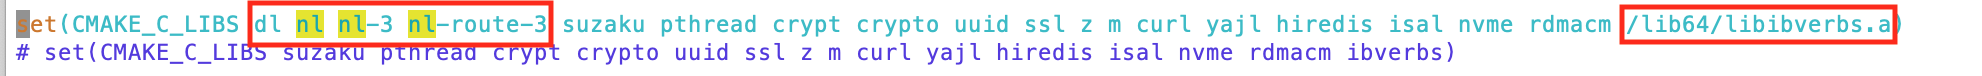
\includegraphics[width=10cm]{../imgs/cmake-link-static.png}
\end{center}

生成静态库
\begin{myeasylist}{itemize}
& SHARED  -> STATIC
& LIBRARY -> ARCHIVE
\end{myeasylist}

\section{gdb}

\begin{myeasylist}{itemize}
& ~/.gdbinit
& info registers
& info sharedlibrary
& gdb -p
\end{myeasylist}

gdb -p发现了mbuffer\_writefile进入死循环,原因是count==0。

猜想是重入了一个锁。

\section{wireshark}

\chapter{实现}

\section{Schedule}

不能支持嵌套task,用pre yield变量来控制。

\section{内存}

提供什么接口,三种生命周期范围、持久性:
\begin{easylist}[itemize]
& 常驻
& session
& IO
\end{easylist}


使用场景
\begin{easylist}[itemize]
    & core private memory
    & sche\_task
    & RDMA
    & buffer\_t
    && libnvme
    & little object
    & ring
\end{easylist}

采用buddy算法管理连续内存分配

动态化

用面向对象的方式处理,每个core对应一个MR对象。public的也是如此。

每个对象内嵌一个buddy对象管理hugepage的分配、释放。
另外,从core的MR里,利用buddy算法分配连续内存,用于ring等小对象。

禁止在一个core内malloc,由另外一个core进行free。

怎么抽象一般内存和hugepage-based内存?

抽象出head,core和public重用代码。第一选择head,第二执行head的操作。

\subsection{buffer}

\begin{center}
    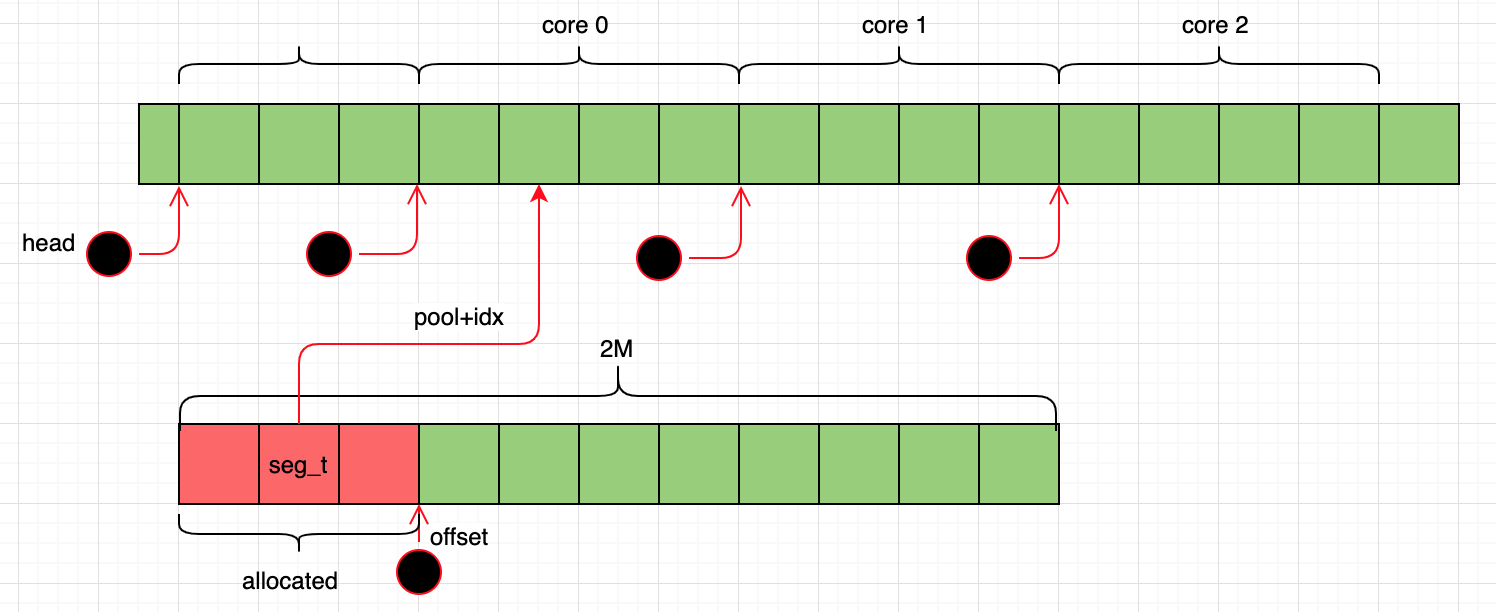
\includegraphics[width=10cm]{../imgs/buffer-t.png}
\end{center}

每个内存区域的\hl{第一个hugepage用来保存该区域的元数据信息},可供分配的是后面的hugepages。
在元数据信息中加上buddy,可用来支持buddy算法。

buffer的每个seg都包含有虚拟地址和物理地址。

\subsection{Memory Pool}

\begin{center}
    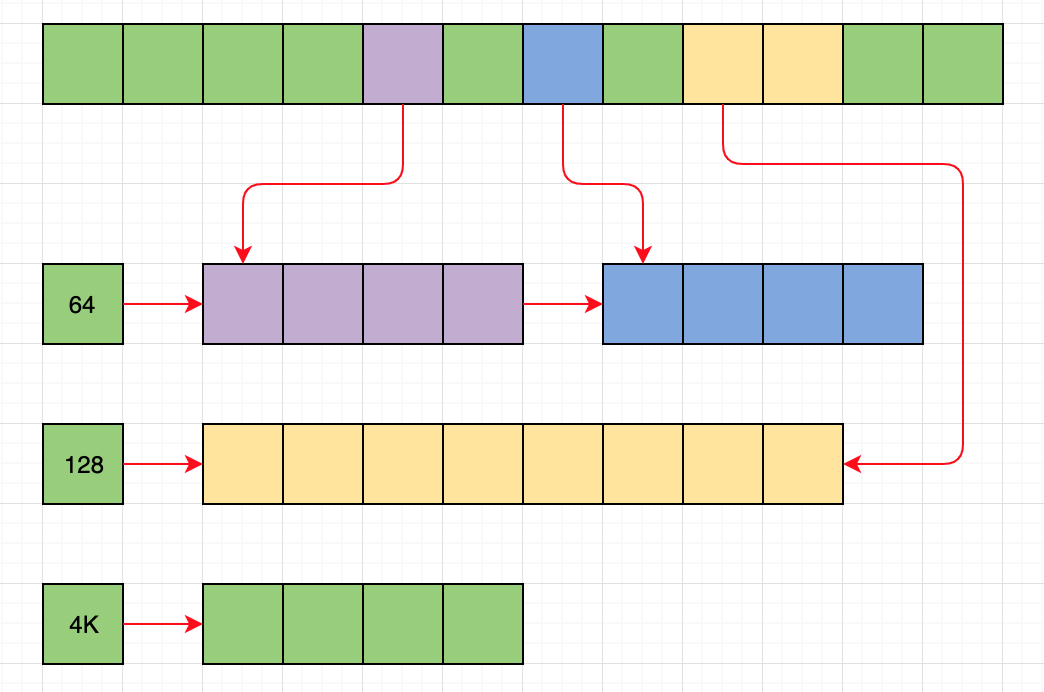
\includegraphics[width=10cm]{../imgs/memory-pool.png}
\end{center}

直接从hugepage申请内存,从hugepage申请一个hugepage,用于小对象。pool管理多个size的小对象队列。
根据要malloc的size,定位到队列。

free时按指针查找属于哪个hugepage。每个hugepge对应起始地址和结束地址以及所在队列的标识。
这样可以保留malloc和free的语法和语义。

hugepage层只需要提供分配单个hugepage的接口,一个队列可以由一个或多个hugepage构成。

或者,memory pool按4k进行组织,同样采用buddy算法。在其上实现ring等。

\hl{每layer都要动态化,包括增和减}。

\subsection{NVMe}

NVMe为什么需要物理地址?

direct io需要512对齐。

\subsection{RDMA}

每个连接$1024*512$内存。

\subsection{IO}

\begin{center}
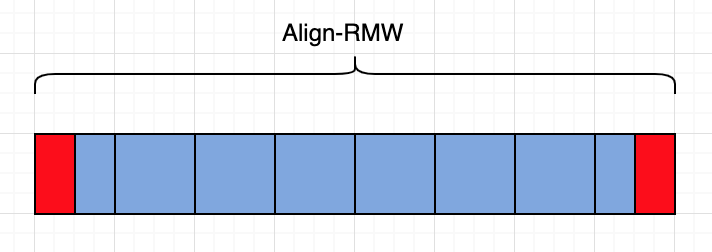
\includegraphics[width=10cm]{../imgs/io-align.png}
\end{center}

首尾页对齐

buffer\_t包含一个seg时,方便处理。如果有多个seg,是否需要分配连续的大块内存。

\hl{SPDK的大IO问题}:NVMe需要物理内存,并且一次io物理内存是连续的。
malloc的内存,不容易找到物理内存。
2M的hugepage虽然能获取虚拟地址连续的4M地址空间,但底层物理内存未必连续。
用1G的hugepage更容易管理。

GFM的机制是什么?barrier去解决RMW、chunk恢复等问题?


\end{document}
